\documentclass{article}

\usepackage[margin=1in]{geometry}
\usepackage{wrapfig}
\usepackage{tkz-euclide}
\usepackage{csquotes}
\usepackage{hyperref}
\usepackage{graphicx}
\usepackage{siunitx}

\title{2021 Castro Valley Junior Math Tournament Problems}
\author{}
\date{}

\begin{document}
\maketitle

\section*{Look Mom No Proof!}
Bessie the Cow found a website called \url{vixra.org} which mostly publishes scientific nonsense.
There's a paper (\url{https://vixra.org/abs/2008.0229}) which presents a simple method that supposedly checks whether integers greater than $5$ are prime.
It makes the following statement without proof:
\begin{displayquote}
    The answer to whether the given numbers are prime numbers is to check that:
    \begin{itemize}
        \item[a)] The numbers are not even numbers (the last digit is not divisible by $2$);
        \item[b)] The last digit of numbers in not $5$;
        \item[c)] The sum of the digits of each of the remaining numbers is not divisible by $3$.
    \end{itemize}
    A number that meets the above criteria is either a prime or a power [of a] prime.
\end{displayquote}
Disprove this claim.

\section*{Mooish}
Farmer Paul has two types of cows: truthy cows and falsy cows.
Physically, they are indistinguishable.
They all speak mooish, and they can be distinguished by how they answer questions.
The truthy cows always reply truthfully, and the falsy cows always lie.
Bessie had a conversation with three of Farmer Paul's cows: Annabelle, Betsie, and Cornelius.
Here's a translation of the conversation.
\begin{displayquote}
	Bessie: Annabelle, is Betsie truthy or falsy? \\
	Annabelle: Falsy \\
	Bessie: Betsie, are the types of Annabelle and Cornelius different? \\
	Betsie: No. \\
	Bessie: Talkative lot, aren't they? Cornelius, is Betsie truthy or falsy? \\
	Cornelius: Truthy.
\end{displayquote}
What is the type of each cow?

\section*{Green Cows}
Help Bessie the Cow answer the question ``How much grass can a green cow chow if green cows can chow grass?''
Bessie and Elsie both chow grass at constant rates.
If Bessie can chow all the grass in a field in $3$ hours and Elsie can chow all the grass in the same field in $4$ minutes, how long will it take for them to chow all the grass in this field together?
Express your answer in exact form.

\section*{Moodern Art}
\begin{wrapfigure}{r}{0.35\linewidth}
	\vspace{-20pt}
	\centering
	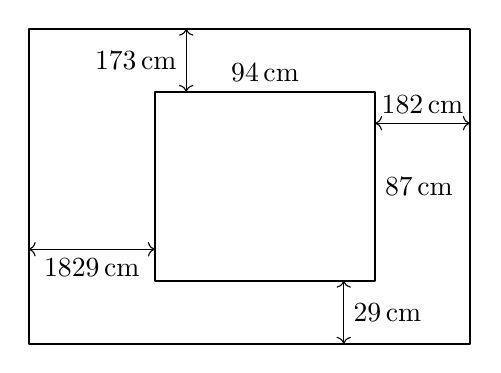
\begin{tikzpicture}[scale=0.8]
		\tkzDefPoint(0,0){A}
		\tkzDefPoint(0,5){B}
		\tkzDefPoint(7,5){C}
		\tkzDefPoint(7,0){D}
		\tkzDrawPolygon[thick](A,B,C,D)

		\tkzDefPoint(2,1){E}
		\tkzDefPoint(2,4){F}
		\tkzDefPoint(5.5,4){G}
		\tkzDefPoint(5.5,1){H}
		\tkzDrawPolygon[thick](E,F,G,H)
		\tkzLabelSegment[above](F,G){$\SI{94}{cm}$}
		\tkzLabelSegment[right](G,H){$\SI{87}{cm}$}

		\tkzDefPoint(0,1){I}
		\tkzDefPoint(2,5){J}
		\tkzDefPoint(7,4){K}
		\tkzDefPoint(5.5,0){L}
		\tkzDrawSegment[thin,arrows=<->]([yshift=0.5cm]E,[yshift=0.5cm]I)
		\tkzLabelSegment[below]([yshift=0.5cm]E,[yshift=0.5cm]I){$\SI{1829}{cm}$}
		\tkzDrawSegment[thin,arrows=<->]([xshift=0.5cm]F,[xshift=0.5cm]J)
		\tkzLabelSegment[left]([xshift=0.5cm]F,[xshift=0.5cm]J){$\SI{173}{cm}$}
		\tkzDrawSegment[thin,arrows=<->]([yshift=-0.5cm]G,[yshift=-0.5cm]K)
		\tkzLabelSegment[above]([yshift=-0.5cm]G,[yshift=-0.5cm]K){$\SI{182}{cm}$}
		\tkzDrawSegment[thin,arrows=<->]([xshift=-0.5cm]H,[xshift=-0.5cm]L)
		\tkzLabelSegment[right]([xshift=-0.5cm]H,[xshift=-0.5cm]L){$\SI{29}{cm}$}
	\end{tikzpicture}
	\vspace{-20pt}
\end{wrapfigure}
Bessie the Cow created a new painting.
It is in the shape of a rectangle $87$ centimeters tall and $94$ centimeters wide.
She hangs it on a rectangular wall such that the top edge of the painting is $173$ centimeters away from the top edge of the wall, the left edge of the painting is $1829$ centimeters away from the left edge of the wall, the right edge of the painting is $182$ centimeters away from the right edge of the wall, and the bottom edge of the painting is $29$ centimeters away from the bottom edge of the wall.
What is the area of the part of the wall that is not covered by the painting?

\section*{Cowld}
\begin{wrapfigure}{r}{0.35\linewidth}
    \vspace{-20pt}
    \centering
	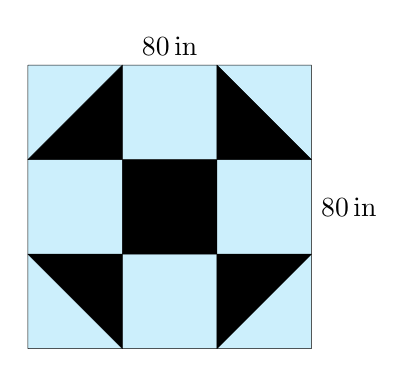
\begin{tikzpicture}[scale=0.4]
		\tkzDefPoint(0,0){A}
		\tkzDefPoint(9,0){B}
		\tkzDefSquare(A,B)
		\tkzGetPoints{C}{D}
		\tkzDrawPolygon[fill=cyan!20](A,B,C,D)
		\tkzLabelSegment[above](C,D){$\SI{80}{in}$}
		\tkzLabelSegment[right](B,C){$\SI{80}{in}$}

		\tkzDefPoint(3,3){E}
		\tkzDefPoint(6,3){F}
		\tkzDefSquare(E,F)
		\tkzGetPoints{G}{H}
		\tkzDrawPolygon[fill=black](E,F,G,H)
		
		\tkzDefPoint(3,0){I}
		\tkzDefPoint(6,0){J}
		\tkzDefPoint(9,3){K}
		\tkzDefPoint(9,6){L}
		\tkzDefPoint(6,9){M}
		\tkzDefPoint(3,9){N}
		\tkzDefPoint(0,6){O}
		\tkzDefPoint(0,3){P}
		\tkzDrawPolygon[fill=black](E,I,P)
		\tkzDrawPolygon[fill=black](F,J,K)
		\tkzDrawPolygon[fill=black](G,L,M)
		\tkzDrawPolygon[fill=black](H,N,O)
	\end{tikzpicture}
	\vspace{-20pt}
\end{wrapfigure}
Cowboy Alex wants to make a blanket for his cows with a specific pattern because they are cold.
If the blanket uses the pattern $36$ times and one side of the pattern is $80$ inches, at least how many inches of black fabric will he need to make blankets for $20$ cows?

\section*{Moocraft}
Bessie the Cow's new hobby is trying to beat the video game Moocraft as fast as possible.
On the first day, Bessie finished Moocraft in $40$ minutes.
The next day, Bessie finished Moocraft in three-fourths of the time it took the day before.
On the third day, Bessie's time is five-sevenths of the time on the second day.
How many seconds did it take for Bessie to complete Moocraft on the third day?
Round your answer to the nearest integer.

\section*{Crack the Cowde}
Bessie the Cow isn't very good at cybersecurity!
She made the password to her Moocraft account only three numerical digits long.
No digit is 0.
The hundreds digit is a multiple of 4, the tens digit is a perfect square, and the ones digit is a multiple of 3.
The digits are in decreasing order.
What is Bessie's Moocraft password?

\section*{Moorio Kart}
Cowboy Alex gave Bessie the Cow a new racing game called Moorio Kart!
She let all one hundred of her cow friends play, and then asked each cow whether they liked each of the three courses.
$65$ cows said they liked Bowser's Cowstle, $75$ cows said they liked Cowconut Mall, and $85$ cows said they liked Moo Moo Meadows.
What is the fewest number of cows that could have said they liked all three courses?

\section*{Cownt the Rectangles}
\begin{wrapfigure}{r}{0.35\linewidth}
	\vspace{-20pt}
	\centering
	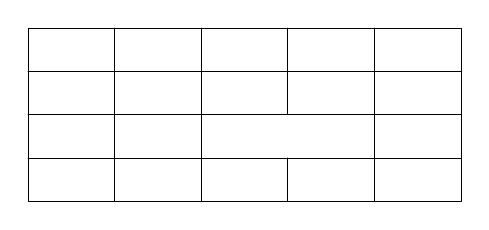
\begin{tikzpicture}[scale=0.55]
		\tkzDefPoint(0,0){A}
		\tkzDefPoint(0,4){B}
		\tkzDefPoint(10,4){C}
		\tkzDefPoint(10,0){D}
		\tkzDrawPolygon(A,B,C,D)

		\tkzDefPoint(0,1){E}
		\tkzDrawSegment(E,[xshift=10cm]E)
		\tkzDefPoint(0,2){F}
		\tkzDrawSegment(F,[xshift=10cm]F)
		\tkzDefPoint(0,3){G}
		\tkzDrawSegment(G,[xshift=10cm]G)

		\tkzDefPoint(2,0){H}
		\tkzDrawSegment(H,[yshift=4cm]H)
		\tkzDefPoint(4,0){I}
		\tkzDrawSegment(I,[yshift=4cm]I)
		\tkzDefPoint(6,0){J}
		\tkzDrawSegment(J,[yshift=1cm]J)
		\tkzDrawSegment([yshift=2cm]J,[yshift=4cm]J)
		\tkzDefPoint(8,0){K}
		\tkzDrawSegment(K,[yshift=4cm]K)
	\end{tikzpicture}
	\vspace{-20pt}
\end{wrapfigure}
Bessie the Cow found a piece of paper with the following figure printed on it.
She wants to know how many rectangles are in the figure.
Help her by finding the number of rectangles of any size that is in this figure, including rectangles which contain multiple smaller rectangles.

\section*{Moogic}
\begin{wrapfigure}{r}{0.35\linewidth}
	\vspace{-20pt}
	\centering
	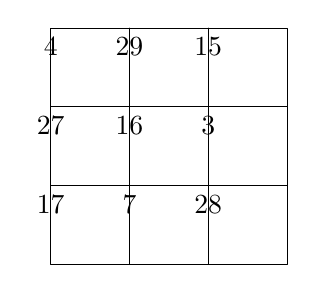
\begin{tikzpicture}
		\tkzDefPoint(0,0){A}
		\tkzDefPoint(3,0){B}
		\tkzDefSquare(A,B)
		\tkzGetPoints{C}{D}
		\tkzDrawPolygon(A,B,C,D)

		\tkzDefPoint(1,3){E}
		\tkzDefPoint(2,3){F}
		\tkzDrawSegment(E,[yshift=-3cm]E)
		\tkzDrawSegment(F,[yshift=-3cm]F)

		\tkzDefPoint(0,2){G}
		\tkzDefPoint(0,1){H}
		\tkzDrawSegment(G,[xshift=3cm]G)
		\tkzDrawSegment(H,[xshift=3cm]H)

		\tkzDefPoint(1,2){J}
		\tkzDefPoint(2,2){K}
		\tkzDefPoint(1,1){L}
		\tkzDefPoint(2,1){M}

		\foreach \name\value in {D/$4$, E/$29$, F/$15$, G/$27$, J/$16$, K/$3$, H/$17$, L/$7$, M/$28$}
		{
			\tkzLabelPoint(\name){\value}
		}


	\end{tikzpicture}
	\vspace{-20pt}
\end{wrapfigure}
Bessie the Cow wanted to learn how to do magic, but she got distracted on the internet and ended up learning about magic squares.
In a magic square, the sum of the numbers in each row, each column, and the two main diagonals are the same.
If exactly two numbers are changed in this grid, the result is a magic square.
Which two numbers must be changed and what values should they be changed?

\section*{Green Cows 2}
Bessie the Cow still hasn't figured out how much grass a green cow can chow if green cows can chow grass.
If $5$ green cows can chow $8$ square meters of grass in $20$ minutes, how many green cows are needed to chow $\SI{10}{m^2}$ of grass in $15$ minutes?
Assume that all green cows in this problem chow grass at the same constant rate.

\section*{Cowlifornia}
Bessie the Cow and her siblings have always dreamed of living in Cowlifornia.
However, Bessie has a lot of siblings, so it'll be hard to find a farm they van all moove to!
Bessie has two more sisters than brothers.
Her brother, Kiran, has twice as many sisters as brothers.
How many siblings does Bessie have?

\section*{Cowkies}
When Bessie the Cow was visiting a nearby farm, she noticed that there was a large herd of cows.
She brought some cookies to make new cow friends, but she didn't know how many cows there were in the group!
She counted a total of $87$ black spots $83$ white spots.
Each cow either has two black spots and three white spots or three black spots and two white spots.
How many cows are in the group, excluding Bessie?

\section*{Moo York Bagels}
Bessie the Cow now lives in Moo York.
As a young country-born-and-raised heifer, she feels a bit homesick and misses her local cuisine.
Luckily, she discovered Billie's Bagel Business.
Every day, she selects a bagel based on her mood.
If Bessie is happy, she will spend \$$1,000$ on a toasted blueberry bagel.
If Bessie is sad, she will spent \$$620$ on a strawberry cream cheese bagel.
On any given day, Bessie has a $68\%$ chance of being happy.
On average, how much does Bessie spend on the bagels each day?
Round your answers to the nearest cent.

\section*{On the Moove}
Bessie the Cow and her sister Bailey the Cow leave their barn at the same time, running at a constant speed on a narrow and straight road.
Bessie went northbound traveling at $42$ miles per hour.
After $2$ hours, Bessie and Bailey are $30$ miles apart.
What was Bailey's speed in miles per hour?

\section*{Farmer Pearson's Pears}
Cowboy Alex just ran out of fresh fruit!
He decided to visit Farmer Pearson for some of his world-famous pears.
Farmer Pearson puts together $18$ pears in one pack and he only sells whole packs.
If Cowboy Alex wants to buy at least five dozen pears, how many packs does he need to buy at the minimum?

\section*{Soccow Tournament}
Rancher Cedric decided to hold a soccow tournament for his cows.
Bessie the Cow's team, the Tactful Tauruses, lost $7$ or their first $9$ games.
However, Bessie decided that she wasn't going to accept losing anymore, and encouraged her team to work harder
Bessie's team ended up winning $75\%$ of their remaining games.
They had victories in exactly $\frac{2}{3}$ of all their games.
In all, how many games did the Tactful Tauruses win?
\end{document}
